\documentclass[11pt,fleqn]{practice}

% Comente a linha seguinte para incluir as soluções
\tcbset{lowerbox=ignored}

\begin{document}

\institution{UFOP\quad DECOM}
\course{Programação de Computadores I}
\subtitle{Aula prática 3}
\title{Comandos de Desvio 1}
\author{}
\date{2014--2}
\maketitle


\begin{abstract}
  Nesta aula você irá resolver problemas que requerem uma decisão com
  base em um teste, ou condição. Para implementar a solução de problemas
  desse tipo, são utlizados comandos de desvio do fluxo de execução do
  programa (\textbf{if-then-else}).
\end{abstract}

\tableofcontents

\section{Comando de desvio}

Suponha que você quer escrever um programa Scilab para calcular o valor
de $f(x)$, onde $f$ é a função definida a seguir, e $x$ é um valor
especificado pelo usuário.
\[ f(x) = \ln \frac{1}{1-x}\]
Note que essa função não é definida se $x=1$. Portanto, seu programa
deverá testar se o valor especificado pelo usuário é igual a 1 e, em
caso afirmativo, informar ao usuário que esse não é um valor
válido. Caso contrário, o programa deve calcular e imprimir o valor de
$f(x)$.

O programa poderia ser então escrito do seguinte modo:
\begin{lst}{scilab}
x = input("Informe o valor de x (deve ser diferente de 1): ")
if x <> 1 then 
    printf("f(%g) = %g\n", x, 1/log(1-x))
else 
    printf("Valor inválido: deve ser diferente de 1\n")
end
\end{lst} 

Um comando \textbf{if-then-else} tem a seguinte sintaxe:

\begin{tabbing} xxxxxxxxxxxxxxxx\=ifxx\= \+\kill
      \textbf{if}  \emph{condição} \textbf{then} \\
	   \>\emph{bloco de comandos 1} \\
     \textbf{else} \\
	   \> \emph{bloco de comandos 2} \\
     \textbf{end}
\end{tabbing}

A \emph{condição} deve ser uma expressão \emph{lógica}
(\emph{booleana}), isto é, uma expressão cujo valor é verdadeiro
(\texttt{\%t}) ou é falso (\texttt{\%f}). Cada bloco de comandos é uma
sequência de comandos, incluindo, possivelmente, outros comandos de
desvio.

A execução de um comando \textbf{if-then-else} é feita do seguinte modo:
primeiro, a condição é avaliada; se o valor resultante for \texttt{\%t},
o bloco de comandos 1 é executado; caso contrário (se o valor for
\texttt{\%f}), o bloco de comandos 2 é executado.

\emph{Observação\/}: a parte \textbf{else} do comando pode ser omitida,
caso não se deseje executar nenhum comando particular no caso em que a
condição seja falsa.

\section{Operações relacionais}


Expressões lógicas podem ser construídas usando-se \emph{operadores
  relacionais\/} (tal como \texttt{<} ou \texttt{<=}), e podem ser
combinadas por meio de \emph{operadores lógicos\/}, tais como
\texttt{\&} e \texttt{|}. Os operadores relacionais e os operadores
lógicos disponíveis em Scilab são mostrados nas tabelas a seguir.

\begin{center}
  \begin{tabular}{p{2cm}l} \hline
    \multicolumn{2}{c}{\textbf{Operadores Relacionais}} \\\hline
    \textbf{operação} & \textbf{descrição} \\\hline
    \texttt{$x$ < $y$}      & $x$ menor que $y$ \\\hline
    \texttt{$x$ <= $y$}    & $x$ menor ou igual a $y$ \\\hline
    \texttt{$x$ > $y$}      & $x$ maior que $y$ \\\hline
    \texttt{$x$ >= $y$}    & $x$ maior ou igual a $y$ \\\hline
    \texttt{$x$ == $y$}    & $x$ igual a $y$ \\\hline
    \texttt{$x$ \textasciitilde= $y$}\newline \texttt{$x$ <> $y$}  & $x$ diferente de $y$ \\\hline
  \end{tabular}
\end{center}

\begin{center}
  \begin{tabular}{p{2cm}ll} \hline
    \multicolumn{3}{c}{\textbf{Operadores Lógicos}}                                                                  \\\hline
    \textbf{operação}            & \textbf{descrição} & \textbf{semântica}                                           \\\hline
    \texttt{\textasciitilde $b$} & negação (não)      & verdadeira se e somente se $b$ é falsa                       \\\hline
    \texttt{$b1$ \& $b2$}        & conjunção (e)      & verdadeira se e somente se $b1$ e $b2$ são ambas verdadeiras \\\hline  
    \texttt{$b1$ | $b2$}         & disjunção (ou)     & falsa se e somente se $b1$ e $b2$ são ambas falsas           \\\hline
  \end{tabular}
\end{center}

\section{Validação de dados}

Muitas vezes os dados informados pelo usuário em uma aplicação precisam
ser validados antes de serem usados. Isto pode ser feito usando um
comando condicional, como é ilustrado no exemplo a seguir.

Para verificar se um número é inteiro, converta-o para o tipo inteiro
usando a função \texttt{int} e verifique se o resultado é igual ao
número original.

Para verificar se um número é natural, verifique se ele é inteiro e não
negativo.

Por exemplo, o programa seguinte obtem um número natural e faz a
validação do mesmo.
\lstinput{scilab}{listings/p03/validacao1.sce}

Veja uma outra maneira de fazer a mesma validação:
\lstinput{scilab}{listings/p03/validacao2.sce}

\begin{runexample}
digite um número natural: 45
número válido: 45
\end{runexample}

\begin{runexample}
digite um número natural: 2.34
número inválido
\end{runexample}

\begin{runexample}
digite um número natural: -67
número inválido
\end{runexample} 

\begin{runexample}
digite um número natural: -0.25
número inválido
\end{runexample}


\section{Problemas}

\begin{task}[breakable]{Fechamento de notas}{}
  Escreva um programa que leia quatro notas de um aluno, calcule e
  mostre a média aritmética das notas e a mensagem de \emph{aprovado} ou
  \emph{reprovado}, considerando que para aprovação é necessária a média
  mínima de sete.

  Não é necessário fazer a validação dos dados de entrada.

  \begin{runexample}
RESULTADO DAS NOTAS
-------------------
nota 1: 8.1
nota 2: 9.8
nota 3: 6.9
nota 4: 7.5
a média aritmética das notas é 8.075
aprovado
  \end{runexample}

  \begin{runexample}
RESULTADO DAS NOTAS
-------------------
nota 1: 6.75
nota 2: 5.2
nota 3: 7
nota 4: 4.5
a média aritmética das notas é 5.8625
reprovado
  \end{runexample}

  \tcblower
  \solution
  \lstinput{scilab}{listings/p03/media.sce}
\end{task}

\begin{task}[breakable]{Ternos pitagóricos}{}
  Em Matemática, nomeadamente em Teoria dos Números, um terno pitagórico
  (ou trio pitagórico, ou ainda tripla pitagórica) é formado por três
  números naturais $a$, $b$ e $c$ tais que $a^2+b^2=c^2$. O nome vem do
  teorema de Pitágoras, que afirma que se as medidas dos lados de um
  triângulo retângulo são números inteiros, então são um terno
  pitagórico.

  Codifique um programa que leia três números naturais e verifique se
  representam um terno pitagórico.

  Caso os valores digitados pelo usuário não sejam números naturais, o
  programa deve apresentar uma mensagem indicando que os valores são
  inválidos.

  \begin{runexample}
Verificação de ternos pitagóricos
------------------------------------------
Digite o valor de a: 3
Digite o valor de b: 4
Digite o valor de c: -5.6
Valores inválidos!
  \end{runexample}

  \begin{runexample}
Verificação de ternos pitagóricos
------------------------------------------
Digite o valor de a: 3
Digite o valor de b: 4
Digite o valor de c: 5
3, 4 e 5 representam um terno pitagórico
  \end{runexample}

  \begin{runexample}
Verificação de ternos pitagóricos
------------------------------------------
Digite o valor de a: 2
Digite o valor de b: 2
Digite o valor de c: 10
Os valores não representam um terno pitagórico
  \end{runexample}

  \tcblower
  \solution
  \lstinput{scilab}{listings/p03/ternos-pitagoricos.sce}
\end{task}

\begin{task}[breakable]{Peso ideal}{}
  Segundo uma tabela médica, o peso ideal de uma pessoa está relacionado
  com a altura e o sexo da pessoa, como mostra a tabela a seguir.

  Fazer um programa que receba como entradas a altura e o sexo; a seguir
  ele calcula e imprime o peso ideal dessa pessoa, utilizando as
  seguintes fórmulas:
  \begin{center}
    \begin{tabular}{ll} \hline
      \textbf{sexo} & \textbf{peso ideal}    \\\hline
      masculino     & $72.7 \times h - 58$   \\
      feminino      & $62.1 \times h - 44.7$ \\ \hline
    \end{tabular}
  \end{center}
  onde $h$ é a altura da pessoa.

  O programa deve verificar se os dados são válidos, ou seja, se a
  altura não é negativa e o sexo é \emph{m} ou \emph{f}.

  Veja a seguir ilustrações de entradas e saídas de execuções do
  programa.

  \begin{runexample}
Cálculo do peso ideal
------------------------------------------
Qual é a altura (em metros)? -1.4
Qual é o sexo (m/f)? m
Dados inválidos!
  \end{runexample}

  \begin{runexample}
Cálculo do peso ideal
------------------------------------------
Qual é a altura (em metros)? 1.72
Qual é o sexo (m/f)? h
Dados inválidos!    
  \end{runexample}

  \begin{runexample}
Cálculo do peso ideal
------------------------------------------
Qual é a altura (em metros)? 1.65
Qual é o sexo (m/f)? f
O peso ideal é 57.765 kg
  \end{runexample}

  \begin{runexample}
Cálculo do peso ideal
------------------------------------------
Qual é a altura (em metros)? 1.8
Qual é o sexo (m/f)? m
O peso ideal é 72.86 kg
  \end{runexample}

  \tcblower
  \solution
  \lstinput{scilab}{listings/p03/peso-ideal.sce}
\end{task}

\begin{task}[breakable]{Quantidade de ladrilhos}{}
  Um pedreiro precisa calcular quantos ladrilhos de cerâmica ele deve
  comprar para cobrir a área de uma sala. Faça um programa que leia a
  área da sala (em cm$^2$), e o tipo de ladrilho a ser adquirido, e
  calcule e imprima o número de ladrilhos necessários. As áreas de cada
  um dos tipos de ladrilhos disponíveis são dadas na tabela abaixo:

  \begin{center}
    \begin{tabular}{ll} \hline
      \textbf{tipo do ladrilho} & \textbf{área de uma peça (cm$^2$)} \\\hline
      1                         & 80                                 \\
      2                         & 60                                 \\
      3                         & 40                                 \\ \hline
    \end{tabular}
  \end{center}

  \begin{runexample}
Cálculo da quantidade de peças de ladrilho
------------------------------------------
Área da sala (em cm^2): 820
Tipo do ladrilho (1/2/3): 1

Quantidade de ladrilhos necessários: 11
  \end{runexample}

  \begin{runexample}
Cálculo da quantidade de peças de ladrilho
------------------------------------------
Área da sala (em cm^2): 820
Tipo do ladrilho (1/2/3): 2

Quantidade de ladrilhos necessários: 14
  \end{runexample}

  \begin{runexample}
Cálculo da quantidade de peças de ladrilho
------------------------------------------
Área da sala (em cm^2): 820
Tipo do ladrilho (1/2/3): 3

Quantidade de ladrilhos necessários: 21
  \end{runexample}

  \begin{runexample}
Cálculo da quantidade de peças de ladrilho
------------------------------------------
Área da sala (em cm^2): -500
Tipo do ladrilho (1/2/3): 8

Dados inválidos!
  \end{runexample}

  \paragraph{Dica}
  Os dados serão inválidos quando:
  \begin{itemize}
    \item o área for negativa, OU
    \item NÃO for verdade que
    \begin{itemize}
      \item o tipo é 1 OU
      \item o tipo é 2 OU
      \item o tipo é 3
    \end{itemize}
  \end{itemize}
  Codifique esta condição usando os operadores lógicos \verb=|= e
  \verb=~=.

  \tcblower
  \solution
  \lstinput{scilab}{listings/p03/area-ladrilho.sce}
\end{task}

\begin{task}[breakable]{Locação de veículos}{}
  Uma empresa de locação de veículos utiliza os seguintes valores para
  locação de um veículo:
  \begin{itemize}
    \item R\$ 1,20 para os primeiros 100 km rodados,
    \item R\$ 0,80 para os próximos 200 km rodados, e
    \item R\$ 0,70 para a quilometragem acima de 300 km.
  \end{itemize}
  Escreva um programa Scilab que tenha como entrada a quilometragem
  percorrida por um veículo e que calcule e exiba o custo total da
  locação e o custo médio por quilômetro percorrido por esse veículo.

  Veja a seguir exemplos de execução do programa.

  \begin{runexample}
CUSTO DA LOCAÇÃO DE UM VEÍCULO
------------------------------------------
distância percorrida (km): -348
dados inválidos!
  \end{runexample}

  \begin{runexample}
CUSTO DA LOCAÇÃO DE UM VEÍCULO
------------------------------------------
distância percorrida (km): 80
custo total da locação: R$96
custo médio: R$1.2/km
  \end{runexample}

  \begin{runexample}
CUSTO DA LOCAÇÃO DE UM VEÍCULO
------------------------------------------
distância percorrida (km): 150
custo total da locação: R$160
custo médio: R$1.06667/km
  \end{runexample}

  \begin{runexample}
CUSTO DA LOCAÇÃO DE UM VEÍCULO
------------------------------------------
distância percorrida (km): 220
custo total da locação: R$216
custo médio: R$0.981818/km
  \end{runexample}

  \begin{runexample}
CUSTO DA LOCAÇÃO DE UM VEÍCULO
------------------------------------------
distância percorrida (km): 431.6
custo total da locação: R$372.12
custo médio: R$0.862187/km
  \end{runexample}

  \tcblower
  \solution
  \lstinput{scilab}{listings/p03/quilometragem.sce}
\end{task}

% \begin{task}{Tarifa de correio \numex{2.11}}{}
%   O custo de enviar um pacote pelo correio é de R\$ 15,00 para o
%   primeiro kg e R\$ 5,00 para cada meio kg ou fração acima de 1 kg. Se o
%   pacote pesar mais de 35 kg, uma tarifa adicional de R\$ 15,00 é
%   adicionada ao custo. Nenhum pacote com mais de 50 kg é aceito. Escreva
%   um programa que leia o peso do pacote, em kg, e calcule o custo de
%   envio desse pacote.

%   Seu programa deve também testar se o valor informado para o peso do
%   pacote é válido (isto é, se é maior que 0), imprimindo uma mensagem
%   indicativa de \emph{valor inválido}, caso contrário.

%   \emph{OBS\/}: Imprima o custo de envio no formato correto, isto é, com
%   2 casas decimais.

%   \begin{runexample}
% Correios: cálculo da tarifa por pacote
% ---------------------------------------
% Informe o peso do pacote (em kg): 54
% Peso acima do valor permitido 
%   \end{runexample}

%   \begin{runexample}
% Correios: cálculo da tarifa por pacote
% ---------------------------------------
% Informe o peso do pacote (em kg): 3.4
% Custo de envio = 40.00 
%   \end{runexample}

%   \emph{OBS\/}: Teste o seu programa para valores de peso que possam
%   exercitar todos os caminhos de execução do programa, tais como: 1,
%   1.7, 6, 38.2, 50, 54.

%   \tcblower
%   \solution
%   \lstinput{scilab}{listings/p04/tarifa-correio.sce}
% \end{task}

% \begin{task}{Tarifa de Energia }{}
%   A conta de energia elétrica de consumidores residenciais de uma cidade
%   é calculada do seguinte modo, onde o consumo é dado em kilowatts (kw):
%   \begin{itemize}
%     \item Se o consumo é de até 500 kw, a tarifa é de R\$ 0,02 por
%     unidade.
%     \item Se o consumo é maior que 500 kw, mas não excede 1000 kw, a
%     tarifa é de R\$ 0,10 para os 500 primeiros kw e de R\$ 0,05 para
%     cada kw excedente a 500.
%     \item Se o consumo é maior que 1000 kw, a tarifa é de R\$ 0,35 para
%     os 1000 primeiros kw e de R\$ 0,10 para cada kw excedente a 1000.
%     \item Em toda conta, é cobrada uma taxa básica de serviço de R\$
%     5,00, independentemente da quantidade de energia consumida.
%   \end{itemize}

%   Escreva um programa que leia o consumo de energia elétrica de uma
%   residência e imprima a sua conta de energia, no formato indicado no
%   exemplo abaixo. O programa deve verificar se o valor fornecido para o
%   consumo de energia é um valor inteiro positivo e, caso contrário,
%   terminar exibindo uma mensagem indicativa de valor inválido.

%   \begin{runexample}
% Cálculo da Conta de Energia Elétrica
% ------------------------------------
% Informe o consumo de energia: 547
% --------------------------------------
% Consumo                    = 547
% Custo da energia consumida = R$ 304.70
% Tarifa básica de serviço   = R$ 5.00
% Valor a pagar              = R$ 309.70
% -------------------------------------- 
%   \end{runexample}

%   \tcblower
%   \solution
%   \lstinput{scilab}{listings/p04/conta-energia.sce}
% \end{task}

% \newpage
% \begin{task}[breakable]{Refração da Luz \numex{3.12}}{}
%   \emph{Refração\/} é a mudança de direção de uma onda (por exemplo, de
%   luz, ou de som) em razão de uma mudança no seu meio de transmissão,
%   como ilustrado na figura abaixo. Ao passar de um meio 1, com índice de
%   refração $n_1$, para um meio 2, com índice de refração diferente,
%   $n_2$, a frquˆncia da onda permanece a mesma, mas sua velocidade de
%   fase se altera (de $v_1$ para $v_2$), observando-se então uma mudança
%   no ângulo de incidência da onda (de $\theta_1$ para $\theta_2$).  Esse
%   fenômeno é descrito pela chamada \emph{Lei de Snell\/}:
%   \[   \frac{\sin \theta_1}{\sin \theta_2} = \frac{v_1}{v_2} =\frac{n_1}{n_2}  \]

%   \begin{center}
%     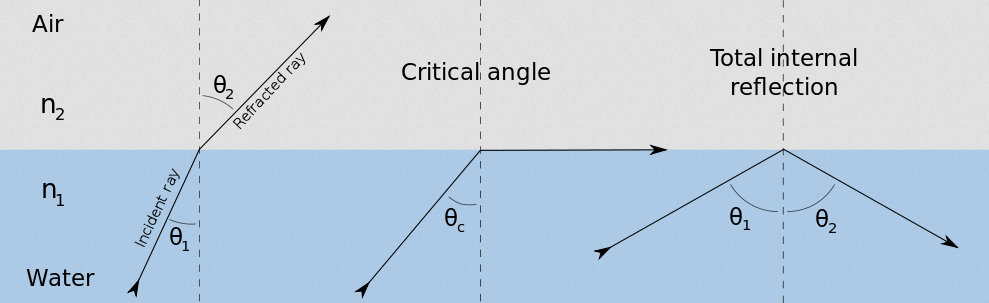
\includegraphics[width=0.9\linewidth]{images/refraction}
%   \end{center}

%   Escreva um programa que leia os índices de refração de dois meios,
%   $n_1$ e $n_2$, e o ângulo de incidência $\theta_1$ (em graus), e
%   calcule e imprima os dados a seguir.
%   \begin{enumerate}
%     \item O ângulo de refração $\theta_2$ correspondente (em graus). Se
%     $(n_1/n_2) \sin \theta_1 > 1$, a equação acima não dará valores
%     reais para $\theta_2$. Neste caso, a onda é toralmente refletida de
%     volta para o meio 1, e o seu programa deverá exibir a mensagem
%     \emph{reflexão total}.

%     \item O ângulo crítico $\theta_c$ (em graus), que é o ângulo de
%     incidência para o qual $\theta_2= 90^o$. Como $\sin(90^o)=1$, o
%     valor do ângulo crítico é $\theta_c=\sin^{-1}(n_2/n_1)$, que somente
%     é definido se $n_2 \leq n_1$. Se o valor do ângulo crítico não for
%     definido, seu programa simplesmente não deverá imprimir tal valor.
%   \end{enumerate}

%   Seu programa deve verificar se os valores fornecidos para os índices
%   de refração $n_1$ e $n_2$ são maiores ou iguais a 1, e também se o
%   valor fornecido para $\theta_1$ está no intervalo $0 \leq \theta_1
%   \leq 90^o$. Caso alguma dessas condições não seja satisfeita, o
%   programa deve terminar, imprimindo a mensagem \emph{valores
%   inválidos}.

%   \begin{runexample}
% Refração de onda 
% ---------------- 
% indice de refração do meio 1 (>= 1) = 1.7
% indice de refração do meio 2 (>= 1) = 1
% ângulo de incidência (0 a 90 graus) = 30
% ângulo de refração = 58.2117 graus 
% ângulo crítico = 36.0319 graus 
%   \end{runexample}

%   \begin{runexample}
% Refração de onda 
% ---------------- 
% indice de refração do meio 1 (>= 1) = 1.7
% indice de refração do meio 2 (>= 1) = 1
% ângulo de incidência (0 a 90 graus) = 45
% reflexão total 
% ângulo crítico = 36.0319 graus 
%   \end{runexample}

%   \begin{runexample}
% Refração de onda 
% ---------------- 
% indice de refração do meio 1 (>= 1) = 1
% indice de refração do meio 2 (>= 1) = 1.7
% ângulo de incidência (0 a 90 graus) = 45
% ângulo de refração = 24.5789 graus 
%   \end{runexample}

%   \tcblower
%   \solution
%   \lstinput{scilab}{listings/p04/refracao.sce}
% \end{task}

% \textbf{\emph{Dicas}}:
% \begin{enumerate}
%   \item Scilab provê funções trigonoétricas para lidar com ângulos
%   expressos em radianos ou em graus. Algumas delas são mostradas na
%   tabela a seguir:

%   \begin{center}
%     \begin{tabular}{p{2cm}l} \hline
%       \textbf{função} & \textbf{descrição} \\\hline
%       \texttt{sin($r$)}      & seno do ângulo $r$, dado em radianos \\\hline
%       \texttt{cos($r$)}     & coseno do ângulo $r$, dado em radianos \\\hline
%       \texttt{asin($x$)}   & valor, em radianos, do ângulo cujo seno é $x$ ($0\leq x \leq 1$) \\\hline
%       \texttt{acos($x$)}   & valor, em radianos, do ângulo cujo coseno é $x$ ($0\leq x \leq 1$) \\\hline
%       \texttt{sind($a$)}     & seno do ângulo $a$, dado em graus \\\hline
%       \texttt{cosd($a$)}      & coseno do ângulo $a$, dado em graus \\\hline
%       \texttt{asind($x$)}     & valor, em graus, do ângulo cujo seno é $x$ ($0\leq x \leq 1$) \\\hline
%       \texttt{acosd($x$)}     & valor, em graus, do ângulo cujo coseno é $x$ ($0\leq x \leq 1$) \\\hline
%     \end{tabular}
%   \end{center}

%   \item Para testar seu programa, você poderá usar alguns dos índices de
%   refração a seguir.

%   \begin{center}
%     \begin{tabular}{p{2cm}l} \hline
%       \textbf{meio} & \textbf{índice de refração} \\\hline
%       \text{vácuo}          & 1.0 \\\hline 
%       \multicolumn{2}{c}{Gases- a $0^o$ C e 1 atm} \\\hline 
%       \text{ar}     & 1.000293 \\\hline
%       \text{hidrogênio}     & 1.000132 \\\hline
%       \multicolumn{2}{c}{Líquidos- a $20^o$ } \\\hline 
%       \text{água}     & 1.3330 \\\hline
%       \text{álcool etílico}     & 1.361 \\\hline
%       \text{benzeno}     & 1.501 \\\hline
%       \multicolumn{2}{c}{Sólidos- temp. ambiente } \\\hline 
%       \text{gelo}            & 1.31 \\\hline
%       \text{quartzo}     & 1.458 \\\hline
%       \text{diamante}     & 2.419 \\\hline
%     \end{tabular}
%   \end{center}

% \end{enumerate}

\end{document}
